\title{2020/03/20 Discussion}
\author{0616014 楊政道}
\maketitle
\thispagestyle{fancy}
\section{Discussion 1}
\subsection{Why do we need to put resistors in the circuit?}
\begin{figure}[!h]
\begin{center} 
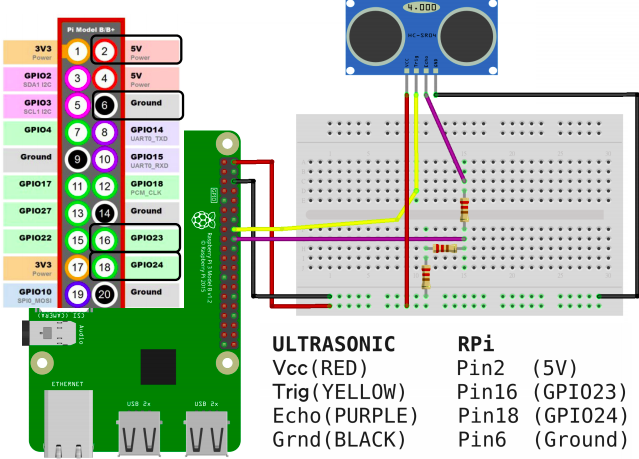
\includegraphics[width=8cm]{resistor.png} 
\caption{resistor layout}
\end{center} 
\end{figure} 
\paragraph{}
Because the output voltage from the \texttt{HC-SR04} Ultrasonic module is \texttt{5V} but the maximum limitation of the voltage to the pin on the raspberrypi is \texttt{3.3V}, we need to reduce the voltage by 3 same resistors to make the voltage into \texttt{5 * 2 / 3 = 3.3V}.
\subsection{Read datasheet. What is the max and min distance that it can detect?}
\begin{figure}[!h]
\begin{center} 
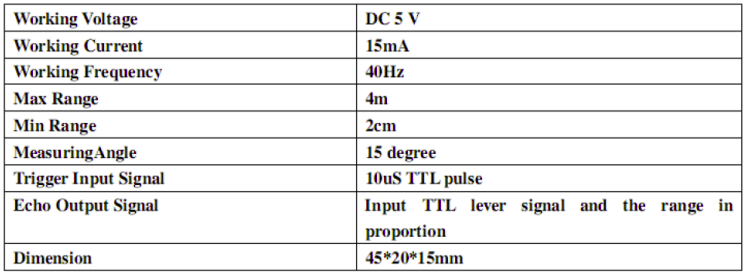
\includegraphics[width=10cm]{HC-SR04-datasheet.png} 
\caption{HC-SR04 datasheet}
\end{center} 
\end{figure} 
\paragraph{}
According to the datasheet of the HC-SR04 module, the maximum range it can detect is 4 meters and the minimun range it can detect is 2 centimeter.
\subsection{Based on distance measurement, is there any other application?}
\begin{figure}[!h]
\begin{center} 
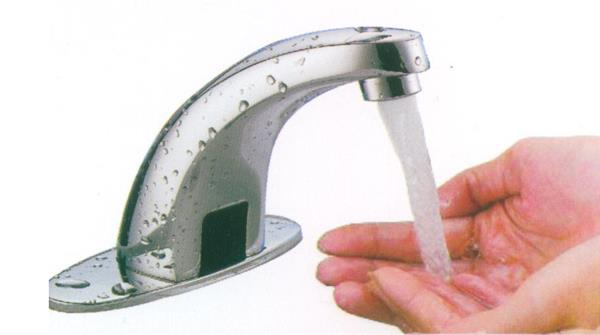
\includegraphics[width=8cm]{faucet.jpeg} 
\caption{induction faucat}
\end{center} 
\end{figure} 
\paragraph{}
One of the applications based on distance measurement is induction faucats. The distance sensor can detect hands are coming and turn the faucet on.
\begin{figure}[!h]
\begin{center} 
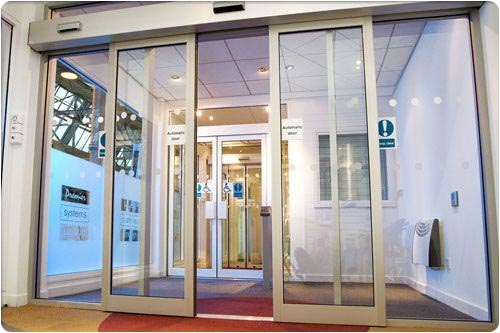
\includegraphics[width=8cm]{automatic-door.jpg} 
\caption{automatic door}
\end{center} 
\end{figure} 
\paragraph{}
Another one of the applications based on distance measurement is automatic door. When someone is close to the door, the door will open.
\subsection{If we want to use Physical PIN number, how to modify the code?}
\section{Discussion 2}
\begin{figure}[!h]
\begin{center} 
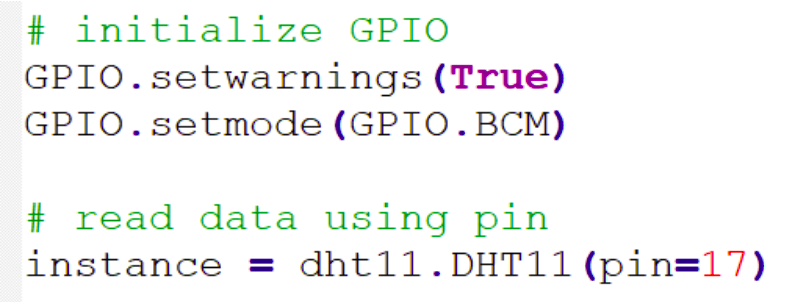
\includegraphics[width=8cm]{sample.png} 
\caption{sample code}
\end{center} 
\end{figure} 
\paragraph{}
We can use \texttt{GPIO.setmode(GPIO.BOARD)} so that we can use physical pin numbers of the raspberry pi.
